\documentclass[11pt,a4paper,dvipdfmx]{article}
%\documentclass[autodetect-engine,dvipdfmx-if-dvi,ja=standard]{bxjsarticle}

\usepackage[utf8]{inputenc}
\usepackage{lmodern}
\usepackage[T1]{fontenc}
\usepackage[noBBpl]{mathpazo}
%\linespread{1.05}
\usepackage{mathtools, amsmath, amssymb, amsthm}
\usepackage{amsfonts}
\usepackage{braket}
%\usepackage{amssymb}
\usepackage{url}
\usepackage{cases}

%% citation
\usepackage[longnamesfirst]{natbib}

%
\theoremstyle{plain}
\newtheorem{thm}{Thm.}[section]
\newtheorem{lem}{Lem.}[section]
\newtheorem{cor}{Cor.}[section]
\newtheorem{prop}{Prop.}[section]
\newtheorem{df}{Def.}[section]
\newtheorem{eg}{e.g.}[section]
\newtheorem{rem}{Rem.}[section]
%

\usepackage{listings,jlisting}
\lstset{%
language={python},%
basicstyle={\ttfamily\footnotesize},%ソースコードの文字を小さくする
frame={single},
commentstyle={\footnotesize\itshape},%コメントアウトの文字を小さくする
breaklines=true,%行が長くなったときの改行。trueの場合は改行する。
numbers=left,%行番号を左に書く。消す場合はnone。
xrightmargin=3zw,%左の空白の大きさ
xleftmargin=3zw,%右の空白の大きさ
stepnumber=1,%行番号を1から始める場合こうする(たぶん)
numbersep=1zw,%行番号と本文の間隔。
}

%\usepackage[dvipdfmx]{graphicx}
%% color packageとdvipdfmxは相性が悪いらしい
%% https://qiita.com/zr_tex8r/items/442b75b452b11bee8049
\usepackage{graphicx}


\usepackage[left=2cm,right=2cm,top=2cm,bottom=2cm]{geometry} %This changes the margins.
\usepackage{float}
%\author{Kyohei Okumura}
\global\long\def\T#1{#1^{\top}}

\newcommand{\id}{\textnormal{id}}
\newcommand{\R}{\mathbb{R}}
\newcommand{\N}{\mathbb{N}}
\newcommand{\Q}{\mathbb{Q}}
\newcommand{\Z}{\mathbb{Z}}
\newcommand{\C}{\mathbb{C}}
\newcommand{\mF}{\mathcal{F}}
\newcommand{\mG}{\mathcal{G}}
\newcommand{\mA}{\mathcal{A}}
\newcommand{\mB}{\mathcal{B}}
\newcommand{\mC}{\mathcal{C}}
\newcommand{\mD}{\mathcal{D}}
\newcommand{\mL}{\mathcal{L}}
\newcommand{\mM}{\mathcal{M}}
\newcommand{\mO}{\mathcal{O}}
\newcommand{\mP}{\mathcal{P}}
\newcommand{\mS}{\mathcal{S}}
\newcommand{\mT}{\mathcal{T}}
\newcommand{\mV}{\mathcal{V}}
\renewcommand{\Re}{\mathrm{Re}}
\renewcommand{\hat}{\widehat}
\renewcommand{\tilde}{\widetilde}
\renewcommand{\bar}{\overline}
\renewcommand{\epsilon}{\varepsilon}
% \renewcommand{\span}{\mathrm{span}}
\newcommand{\defi}{\stackrel{\Delta}{\Longleftrightarrow}}
\newcommand{\equi}{\Longleftrightarrow}
\newcommand{\s}{\succsim}
\newcommand{\p}{\precsim}
\newcommand{\join}{\vee}
\newcommand{\meet}{\wedge}
\newcommand{\1}{\mbox{1}\hspace{-0.25em}\mbox{l}}

\DeclareMathOperator{\Var}{Var}
\DeclareMathOperator{\Cov}{Cov}
\DeclareMathOperator{\sgn}{sgn}
\DeclareMathOperator{\Card}{Card}
\DeclareMathOperator{\supp}{supp}
\DeclareMathOperator{\Log}{Log}
\DeclareMathOperator{\spn}{span}

\newcommand{\indep}{\mathop{\perp\!\!\!\!\perp}}

\usepackage{color}
\newcommand{\kcomment}[1]{{\textcolor{blue}{#1}}}
\newcommand{\ocomment}[1]{{\textcolor{red}{#1}}}


\begin{document}
\title{SML HW3}
\author{29-176004 奥村 恭平{\footnote{E-mail: kyohei.okumura@gmail.com}
\footnote{東京大学大学院 経済学研究科 M2}
}}
\date{\today}
\maketitle

%%%%%%%%%%%%%%%%%%%%%%%%%%%%%%%%%%%%%%%%%%%%%%%%%%%%%%%%%%%

\section*{宿題1}
次の等式を示す.
\begin{equation} \label{goal1}
	E \left. \left[ \hat{\theta} \sum_{i=1}^n \frac{\partial}{\partial \theta} \log q(x_i; \theta) \right|_{\theta = \theta^*} \right] = 1
\end{equation}

$E[\hat{\theta}] = \theta^*$の両辺を$\theta^*$で偏微分することを考える.右辺は1.左辺については,
\begin{align*}
	\frac{\partial}{\partial \theta^*} E[\hat{\theta}(X_1, \dots, X_n)]
	&= \frac{\partial}{\partial \theta^*} \int \hat{\theta}(x_1, \dots, x_n) q(x_1; \theta^*) \cdots q(x_n; \theta^*) dx_1 \cdots dx_n \\
	&= \int \frac{\partial}{\partial \theta^*} \hat{\theta}(x_1, \dots, x_n) q(x_1; \theta^*) \cdots q(x_n; \theta^*) dx_1 \cdots dx_n \quad \text{(微分と積分の順序交換)}\\
	&= \int \hat{\theta}(x_1, \dots, x_n)
	\left.
	\frac{\partial}{\partial \theta}
	\left[
	q(x_1; \theta) \cdots q(x_n; \theta)
	\right]
	\right|_{\theta = \theta^*}
	dx_1 \cdots dx_n
\end{align*}
ここで,
$$
\frac{\partial}{\partial \theta} \log [q(x_1;\theta) \dots q(x_n; \theta)]
=
\frac{\frac{\partial}{\partial \theta} [q(x_1;\theta) \dots q(x_n; \theta)]}{q(x_1;\theta) \dots q(x_n; \theta)}
$$
より,
\begin{align*}
\frac{\partial}{\partial \theta}
\left[
q(x_1; \theta) \cdots q(x_n; \theta)
\right]
&=
\left[
\frac{\partial}{\partial \theta} \log [q(x_1;\theta) \dots q(x_n; \theta)]
\right]
q(x_1;\theta) \dots q(x_n; \theta) \\
&=
\left[
\frac{\partial}{\partial \theta} \sum_{i=1}^n \log q(x_i; \theta)
\right]
q(x_1; \theta) \cdots q(x_n; \theta) \\
&=
\left[
\sum_{i=1}^n \frac{\partial}{\partial \theta} \log q(x_i; \theta)
\right]
q(x_1; \theta) \cdots q(x_n; \theta)
\end{align*}
であるので,

\begin{align*}
\frac{\partial}{\partial \theta^*} E[\hat{\theta}(X_1, \dots, X_n)]
&=
\int \hat{\theta}(x_1, \dots, x_n)
	\left.
	\left[
	\sum_{i=1}^n \frac{\partial}{\partial \theta} \log q(x_i; \theta)
	\right]
	\right|_{\theta = \theta^*}
	q(x_1; \theta^*) \cdots q(x_n; \theta^*)
	dx_1 \cdots dx_n \\
&= E \left. \left[ \hat{\theta} \sum_{i=1}^n \frac{\partial}{\partial \theta} \log q(x_i; \theta) \right|_{\theta = \theta^*} \right]
\end{align*}
となる.よって(\ref{goal1})が示された.
\qed


%%%%%%%%
\newpage
\section*{宿題2}
任意の$i, j \in [n]$について,次の式を示せば良い.
\begin{equation} \label{goal2}
	\int
	\frac{\partial \log q}{\partial \theta_i}(x; \theta)
	\frac{\partial \log q}{\partial \theta_j}(x; \theta)
	q(x; \theta) dx
	=
	- \int \frac{\partial^2 \log q}{\partial \theta_i \partial \theta_j}(x; \theta)
	q(x; \theta) dx
\end{equation}

まず,
\begin{align}
	\frac{\partial^2 \log q}{\partial \theta_i \partial \theta_j}
	&= 
	\frac{\partial }{\partial \theta_i}
	\left(
	\frac{\frac{\partial q}{\partial \theta_j}}{q}
	\right)
	=
	\frac{\partial^2 q}{\partial \theta_i \partial \theta_j} \cdot q^{-1}
	-
	\frac{\partial q}{\partial \theta_j} \frac{\partial q}{\partial \theta_i}q^{-2} \nonumber \\
	&=
	\frac{\partial^2 q}{\partial \theta_i \partial \theta_j} \cdot q^{-1}
	-
	\frac{\partial \log q}{\partial \theta_j} \frac{\partial \log q}{\partial \theta_i} \label{eq2}
\end{align}
である.(\ref{eq2})の第1項について,微分と積分の順序交換を認めると,
$$
\int \frac{\partial^2 q}{\partial \theta_i \partial \theta_j}(x; \theta) q^{-1}(x; \theta) \cdot q(x; \theta) dx
=
\int \frac{\partial^2 q}{\partial \theta_i \partial \theta_j}(x; \theta) dx
= \frac{\partial^2}{\partial \theta_i \partial \theta_j} 
\underbrace{\int q(x; \theta) dx}_{=1}
= 0
$$
となることに注意すれば,(\ref{eq2})の両辺において$x$について積分をとることで,(\ref{goal2})を得る.
\qed



%%%%%%%%%%
\section*{宿題3}
末尾のコード(言語はpython)を用いてシミュレーションした.図中のN\_BERは,最尤推定量一つを求める際にベルヌーイ分布から発生させた標本数,N\_MLEは,最尤推定量の標本数を表す.N\_BERが大きくなると,最尤推定量の分布の形が正規分布の形に近づいていることがわかる.

\begin{figure}[H]
  \centering
    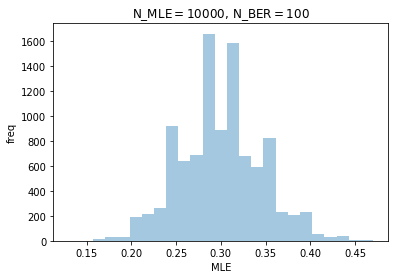
\includegraphics[height=8cm]{image/fig1.png}
    %\caption{\footnotesize $n := 600, \alpha := 0.1$}
    \label{fig:fig1}
\end{figure}
\begin{figure}[H]
  \centering
    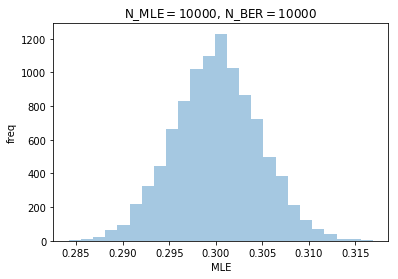
\includegraphics[height=8cm]{image/fig2.png}
    %\caption{\footnotesize $n := 600, \alpha := 0.1$}
    \label{fig:fig2}
\end{figure}

\begin{lstlisting}
import numpy as np
import scipy as sp
from numpy.random import binomial
import matplotlib.pyplot as plt
import seaborn as sns

def mle_sim(N_MLE=100, N_BER=100, theta_true=0.3):
    mle_list = binomial(n=N_BER, p=theta_true, size = N_MLE)/N_BER

    fig = plt.figure()
    ax = fig.add_subplot(1,1,1)
    ax.set_title('N_MLE$ = {0}$, N_BER$ = {1}$'.format(N_MLE, N_BER))
    ax.set_ylabel('freq')
    sns.distplot(mle_list, kde=False, rug=False, bins=25, axlabel="MLE")
    None
\end{lstlisting}


\end{document}